\chapter{智能会话系统中的知识表示和逻辑推理}{Knowledge Representation and Logic Inference for Cognitive Dialogue System}

%%%%%%%%%%%%%%%%%%%%%%%%%%%%%%%%%%%%%%%%%%%%%%%%%
\section{基于超图的知识表示方法}{The Conceptual Model of the Cognitive Dialogue System}
%%%%%%%%%%%%%%%%%%%%%%%%%%%%%%%%%%%%%%%%%%%%%%%%%
XXX简单介绍从语言到逻辑中的语言的几种表现形式;重点论证使用超图来表示语义逻辑的灵活性和高效性等。




%%%%%%%%%%%%%%%%%%%%%%%%%%%%%%%%%%%%%%%%%%%%%%%%%
\section{语言和超图之间的转换之范畴论观}{A Catergory-Theoretic View of Linguistic Hypergraph Transformations}
%%%%%%%%%%%%%%%%%%%%%%%%%%%%%%%%%%%%%%%%%%%%%%%%%
我们的研究目标一直是探讨有关的语言现象和计算系统之间的交集,从而构建具有实用价值的自然语言处理系统,如智能对话系统。后面章节会通过介绍具体实现算法及相关应用来从语用计算语言学角度阐述本文的研究的可行性。本节主要在广泛的数学背景下,语言的范畴论来阐述其理论可行性。

\subsection{Basics of Category Theory}{范畴论的基础知识}

范畴论 \cite{LawvereSchanuel97}常被用于形式化各种数学结构中的共同特性,将这些数学结构的概念形式化成一组组对象和箭头(也称为态射)。一个范畴包括两个基本属性:对象之间的箭头可以复合 ;每个对象有一个标识箭头指向自己。对象和箭头可以是抽象的任何类型,这个简单的结构安排有着非凡的数学能力,使其能被用在探索各个领域的数学理论基础。

形式上,一个范畴包含一下内容:

\begin{itemize}
\item 一个对象类ob(C),其中的元素称为C中的对象。
\item 一个箭头类hom(C),其中的元素称为C中的箭头或态射。hom(a, b)中的元素f称为从a到b的态射,即$f : a \rightarrow b$
\item 一个用于操作态射复合的二元运算子$\circ$, 使得对于ob(C)中的任意三个对象a,b和c,$f : a \rightarrow b$ 和 $g : b \rightarrow c$ 的复合可记为 $g \circ f$ 或 $gf$,并且使得以下两条公理成立:

\begin{itemize}
\item 结合律:如果 $f : a \rightarrow b$, $g : b \rightarrow c$ 和 $h : c \rightarrow d$, 那么 $h \circ (g \circ f) = (h \circ g) \circ f$
\item 同一性:对每一个对象x,存在一个态射 $1x : x \rightarrow x$ 
Identity: For every object x, there exists a morphism $1x : x \rightarrow x$ called the identity morphism for x, such that for every morphism $f : a \rightarrow b$, we have $1b \circ f = f = f \circ 1a$.
\end{itemize}
\end{itemize}

Any directed graph generates a small category: the objects are the vertices of the graph, and the morphisms are the paths in the graph (augmented with loops as needed) where composition of morphisms is concatenation of paths. Such a category is called the free category generated by the graph.

\subsection{A Category-Theoretic View of Linguistic Hypergraph Transformations}

We now explain how the formalism of category theory may be used as a general framework for formalizing and interpreting the diverse linguistic comprehension, generation and reasoning algorithms described in these pages.   The key to this formalization is the OpenCog Atomspace which serves as the common representational framework for these various algorithms.

Let us introduce the term ``t-Atom'' to refer to a triple (Atom, time interval, Atom-state).   In most cases the state of an Atom consists of its TruthValue and its AttentionValue, plus unchanging aspects such as its type and is name.

A 't-Atomspace' associated with an OpenCog system, over a certain interval $T$ of time, consists of the set of t-Atoms $(A,I,S)$ so that

\begin{itemize}
\item A has existed within the OpenCog system's Atomspace at some time point $t \in T$
\item I is an interval between two changes of the state of Atom $A$
\item S is the state of Atom A during interval I
\end{itemize}

Given a t-Atomspace, one can form an 'activity graph' whose nodes are sets of tAtoms, and whose links record activities of cognitive processes that transform the graph.  A link from node $N_1$ to node $N_2$ indicates that a cognitive process has taken $N_1$ as input and given $N_2$ as output.   

Paths through the activity graph result from chaining together cognitive processes.  In category-theoretic terms, the objects here are tAtom-sets, and the morphisms are paths through the activity graph indicating chains of cognitive activity.

For instance:

\begin{itemize}
\item The link parser transforms sets of AdjacencyLinks between WordNodes, into sets of relationships indicating link parser links between these WordNodes.
\item RelEx transforms sets of link parser relationships into sets of relationships indicating semantic relationships.
\item RelEx2Logic transforms sets of relationships output by RelEx, into sets of more abstract relationships more suitable for PLN inference.
\item PLN inference maps Atom-sets into Atom-sets, transforming knowledge extracted from natural language into different forms as suitable for connecting with other knowledge of various sorts.
\item Fuzzy matching, an approach to natural language question-answering (an important ingredient to intelligent dialogue, as described in Chapter \ref{chap:dialogue}) maps an Atom-set into another Atom-set judged as a near match.
\item Microplanning transforms a set $S$ of relationships, intended for articulation, into a new set consisting of a partitioning of $S$ into a subset $S_1$ to be sent to SuReal for articulation, and a subset $S_2$ saved for likely articulation in the near future.
\item Surface realization transforms a set of semantic relationships into a set of link parser relationships; and then transforms a set of link parser relationships into a set of AdjacencyLinks between WordNodes.
\end{itemize}

The comprehension, reasoning/matching and generation processes may thus be viewed very broadly as three  morphisms that can be chained together to form a single morphism corresponding to an instance of linguistic response.

The quality of a response may be quantified by assigning a ``cost'' to each link in the activity graph -- cost being viewed as the opposite of confidence.  Lower confidence in an instance of comprehension, generation or reasoning results in a higher cost to that instance.   The objective of a dialogue system may be viewed as the provision of responses that meet pragmatic goals with the minimum cost in this sense.

A very high level mathematical view of this nature has limited practical utility, in the sense that it does not provide much guidance on which sorts of specific transformation rules are most useful in the context of the details of a particular language like English.   However, it does provide a broader perspective, allowing one to step back from the linguistic particulars and get a clear sense of what sort of operations are being undertaken.   The presentation of comprehension, generation and reasoning as a collection of hypergraph transformations, performed in appropriate sequence, makes clear the role that these linguistic operations play in the broader scope of cognition.

%%%%%%%%%%%%%%%%%%%%%%%%%%%%%%%%%%%%%%%%%%%%%%%%%
\section{概率逻辑网以及基于自然语言的逻辑推理}{Probabilistic Logic Network And Reasoning Based on Natural Language}
\label{sec:pln}
%%%%%%%%%%%%%%%%%%%%%%%%%%%%%%%%%%%%%%%%%%%%%%%%%

XXX本节还要插入基于语言的逻辑推理过程描述以及实例分析(原第5章内容)

在将语言转换成逻辑形式的一个主要目的就是可以进行相应的逻辑推理,本文所采用的逻辑系统是概率逻辑网络PLN。 PLN是一个独特的推理系统,它嵌入了预测逻辑和传统逻辑的组合。PLN在\cite{Goertzel2008, RWR}中被详细介绍。在此我们给出一个高阶的概述。

PLN是一个数学和软件框架,用于非确定推理、操作CogPrime软件框架、使概率真值与泛化逻辑推理规则的整合成为可能。具体来说,PLN包含:

\begin{itemize}
\item 一系列推理规则(例如,演绎、贝叶斯规则、变量归一化、演绎推理,等等),每一项都有一个或多个逻辑关系或词项(以CogPrime的原子来表征)作为输入,并计算输出;
\item 特定的数学方程,基于合适的背景前提假设的概率值,计算结论的概率值。
\end{itemize}
PLN还涉及一条特殊的功能,评估概率值的置信度(证据的分量,或二阶的不确定性)。最后,PLN在软件中的实现需要重要的抉择,要求考虑推理规则的结构化表征、“推理控制”——这种策略要求,在每个特定的实际情况中,判断以何种顺序做何种推理。

\subsection{PLN的一个简单概述}{A Simple Overview of PLN}

PLN的关键因素是它的规则和方程式。总的来说,一个PLN规则有:

\begin{itemize}
\item 输入:一个原子元组(它必须满足某些要求,视规则而定)
\item 输出:一个原子元组
\end{itemize}

实际上,几乎在所有情况下,输出都是一个单一的原子,而输入则是一个单一的原子或者是一对原子。

特定的原形例子是演绎规则,它的输入是这样的:

{\tt\begin{small}\begin{lstlisting}
X_Link A B
X_Link B C
\end{lstlisting}\end{small}}

而它的输出应该是这样的:

{\tt\begin{small}\begin{lstlisting}
X_Link A C
\end{lstlisting}\end{small}}

在这里,X\_Link可以是继承性链接、子集链接、按时链接或延伸按时链接的。

一个PLN方程与一条PLN规则同时存在,它表示了输出的非确定性真值,基于输入的非确定真值。例如,如果我们有:

{\tt\begin{small}\begin{lstlisting}
X_Link A B <sAB>
X_Link B C <sBC>
\end{lstlisting}\end{small}}



那么标准的PLN演绎方程告诉我们

{\tt\begin{small}\begin{lstlisting}
X_Link A C <sAC>
\end{lstlisting}\end{small}}

其中: 

$$
s_{AC}=s_{AB}s_{BC}+\frac{\left(1-s_{AB}\right)\left(s_C-s_Bs_{BC}\right)}{1-s_B}
$$, $s_A$表示节点$A$的真值强度。

在这个例子中,每一个院子的非确定真值通过一个“强度”数值来给出。总的来说,PLN中的非确定真值可以有多种形式,比如:

\begin{itemize}
\item 单一的强度值,比如0.8,这表示概率或模糊真值,取决于具体的原子类型
\item (强度,置信度)对,比如(0.8,0.4)
\item (强度,数量)对,如(0.8,15)
\item 非确定的概率值,如(0.6,0.9, 0.95),这表示概率间的相互评分
\end{itemize}

\subsection{前向和后向链}{Forward and Backward Chaining}

PLN中典型的模式的使用是前向链和后向链推理。

前向链表示:

\begin{enumerate}
\item 给出一个感兴趣的原子池(列表);
\item 应用PLN规则到这些原子上,以产生新的原子,最好也是感兴趣的;
\item 将这些新的原子加如到池中,返回步骤1。
\end{enumerate}

例子:“人是动物”和“动物会吸”是两个池中的原子。它们被演绎规则所组合,形成了结论“人会呼吸”

后向链分为两种情况,第一种:

\begin{itemize}
\item “真值查询”,给出一个原子目标,它的真值未知(或者过于不确定),以及一个原子池,按照演绎规则,通过组合池中原子,找到一种方法来评估该目标原子的真值。
\end{itemize}

例子:目标是“人是否会呼吸?”(继承链接“人会呼吸”)。目标的真值通过“人是动物,动物会呼吸,因此人会呼吸”的推理来评估。

第二种:

\begin{itemize}
\item “填空查询”,给定一个目标链接(原子可以是节点或链接)以及一个或多个目标中间的变量原子,找出什么原子可以被放在变量原子的位置上,可以使目标链接获得一个高的置信度(即一个“高的真值”)。
\end{itemize}

例子:目标是“什么会呼吸”,即“继承链接\$X呼吸”……直接在原子空间中查找发现院子“继承链接 动物会呼吸”,表示空格\$X的位置上可以被填入“动物”。推理揭示“继承链接 人会呼吸”,因此空格\$X也可以被填入“人”。

例子:目标是“什么会呼吸和加法”,即“(继承链接\$X会呼吸)并且(继承链接\$X会加法)”。推理揭示此处\$X可以被填入“人”但不能是“猫”或“电脑”。

常识推理可能涉及一个前向和后向链的组合。

推理中最困难的部分是“推理控制”——在可能的推理步骤中选取哪些步骤,以获得需求的信息(在后向推理中)或获得感兴趣的新信息(在前向推理中)。在一个有大量原子的原子空间中有许多可能的和强大的启发信息需要进行选择。推理控制的最佳指导是某些基于系统的过去推理历史的归纳。当然,一个较信的系统不会有很多的历史信息。依靠非直接的相关历史是一个推理问题——这个问题的最好解决是让系统有一些历史经验。

\subsection{一阶概率逻辑网络}{First Order Probabilistic Logic Networks}

我们以更正式的方式来介绍PLN。PLN被氛围一阶和高阶子理论(FOPLN和HOPLN)。这些词项源自NARS\cite{Wang2006}。我们首先使用了FOPLN,然后他们使用了HOPLN。

FOPLN是一个传统逻辑,设计到词项和词项间的关系(链接)。它是一个非确定逻辑,词项和关系都拥有真值对象,真值对象有多种可能的类型,从单一的数值到复合的结构如非确定概率。词项可以是基本的观察,或一个符号集合$T$中的抽象的符号。

\paragraph{核心FOPLN关系}

“核心FOPLN”涉及集合中的关系:否定、继承、概率合取和析取、成员和模糊合取和析取。基本观察只能有成员链接,而标志词项可以有任何类型的链接。PLN通过链接不同类型的语义来清晰地区分概率关系和模糊集合关系。成员语义通常是模糊关系(尽管它们可能是脆弱的(crisp?),而继承关系是概率性的,并且有规则来管理这二者的互操作。

假定一个虚拟的主体对一个命叫Fluffy的生物做了一次基本的视角观察$o$。这个主体可能将$o$以0.9的隶属度划于“毛皮对象”的模糊集合下,也可能以0.8的隶属度将之划于“动物”的模糊集合下,于是该主体可以在记忆中建立以下链接:

 \begin{tabbing}
\=成员 $o$ 毛皮 $< 0.9 >$ \\
\>成员 $o$ 动物 $< 0.8 >$ \\
\end{tabbing}

随后,该主体可能想要通过合并这些链接来完善它的知识。使用最小化的模糊合取操作,该主体可能会总结出:

 \begin{tabbing}
模糊\=AND\ $<0.8>$\\
\> 成员 $o$ 毛皮 \\
\> 成员 $o$ 动物 \\
\end{tabbing}

这表示对$o$的观察结果是一个毛皮动物对象。

(外部)继承链接的语义与成员链接完全不同,尽管它们是相关的。延伸继承表征一个纯粹的条件概率子集关系,通过子集关系来表达。如果$A$是皮毛的而$B$属于“猫”集合,那么以下陈述:

\begin{tabbing}
\=子集 $<0.9>$\\
\>A\\
\>B\\
\end{tabbing}

意思是:$$P(x \mbox{ 属于集合}\ B\vert x \mbox{ 属于集合}\ A) = 0.9.$$ 

\subsection{PLN 真值}{PLN Truth Values}

为了增加全概率析取的信息量,PLN 拥有一系列不同的真值类型:

\begin{itemize}
\item 强度真值,包含单一数值;例如,$<s>$或$<0.8>$。强度真值通常表示概率,但不总是这样。
\item 单一真值,包括一对数字。这些数字对以以下形式存在:$<s,\ w>$,$s$是一个强度值而$w$是一个“证据的权重值”;$<s,\ N>$,其中$N$是一个“计数”。“证据的权重值”是对信念的量化描述,而“计数”是对重复性证据的量化描述。
\item 非确定性真值,它用区间$[L,U]$、评分水平$b$、以及一个整数$k$来量化对真值的描述。非确定性真值量化了以下的想法:在经过了$k$次观察以后,以概率$b$的可能性,推理的结论会落在区间$[L,U]$中。
\item 分布真值,对整个概率分布的离散化近似。
\end{itemize}

\paragraph{附加的FOPLN关系}

在FOPLN核心关系之上,FOPLN还有两类额外的关系类型。有一类简单的类型,相似度,定义如下:

$$
相似度 \ A \ B
$$

如果$R \ A \ B$ 的真值可以仅仅用核心FOPLN关系中A和B的关系来计算的话,我们把关系$R$叫做简单的。而有一类复杂的“附加”关系,如意向继承(见附录\ref{app:poss_worlds}),描述了与某一词项相关联的模式的属性集合与相应的其他属性集合之间的关系。

回到我们的例子上来,主体可能观察到“猫”的两项属性,即“毛皮”和“会叫”。由于某只哈斯奇也是皮毛动物,主体可能会认为:

{\tt\begin{small}\begin{lstlisting}
意向继承 <0.5>
	哈斯奇  
	猫
\end{lstlisting}\end{small}}

意思是哈斯奇拥有50\%的猫的属性。为了更深入地构建这种关系,PLN还有一个混合的意向/延伸继承关系,简单地通过如子集和意向继承关系的析取来定义。

如例子所陈述,对一个一个复杂的附加关系$R$,$R \ A \ B$的真值是通过一个数值所表达的FOPLN中不同词项的关系的真值来定义的(而不是“$A$而且$B$”),它通过某个特定的数学方程来计算。

\subsection{PLN规则和方程}{PLN Rules and Formulas}

PLN中一个析取是通过规则和方程来达到的。PLN逻辑推理以“三段论演绎规则”的形式进行,以通过合并陈述和匹配的词项来寻找模式。PLN的规则包括但不限于以下例子:

\begin{itemize}
\item deduction $\left((A\rightarrow B) \wedge (B\rightarrow C) \Rightarrow (A\rightarrow C)\right)$,
\item induction $\left((A\rightarrow B) \wedge (A\rightarrow C) \Rightarrow
(B\rightarrow C)\right)$,
\item abduction $\left((A\rightarrow C) \wedge (B\rightarrow C) \Rightarrow
(A\rightarrow C)\right)$,
  \item revision, which merges two versions of the same logical relationship that have different truth values
\item inversion $\left((A\rightarrow B) \Rightarrow
  (B\rightarrow A)\right)$.
\end{itemize}

这些规则的前四项的基本设计如图\ref{fig:inference}所示。我们可以看到前三项规则表示了在三个相关联的词项上做推理的规则,同时还可以看到,归纳和回溯可以从演绎和反向的组合中获得,这是PLN真值公式使用的一项规则。

\begin{figure}[htb]
  \center
  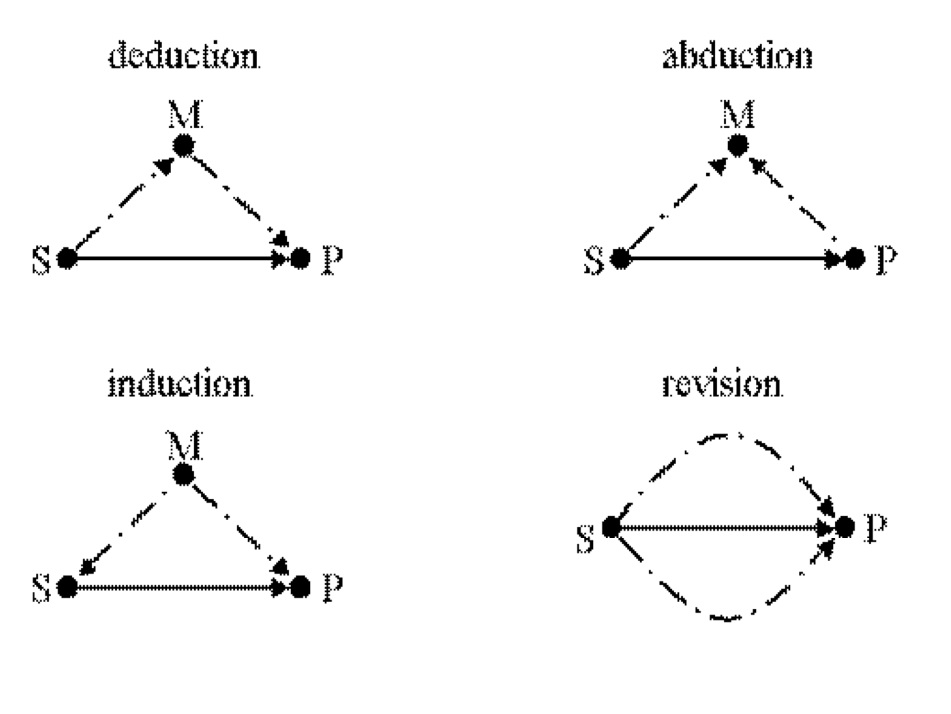
\includegraphics[width=11cm]{figures/inference.png}
  \caption{The four most basic first-order PLN inference rules}
  \label{fig:inference}
\end{figure}

每一项规则都与一个公式相关,它应用规则以计算出真值。例如,假设$s_A$, $s_B$, $s_C$, $s_{AB}$, 以及 $s_{BC}$分别表示词项$A$、$B$、$C$以及关系$A\rightarrow B$和$B\rightarrow C$的真值,那么,在合适的条件下,演绎规则的公式如下:

$$s_{AC}=s_{AB}s_{BC}+\frac{\left(1-s_{AB}\right)\left(s_C-s_Bs_{BC}\right)}{1-s_B},$$

其中$s_{AC}$表示关系$A\rightarrow C$的真值,这个公式的前提是,假设$A\rightarrow B$和$B\rightarrow C$是相互独立的。

对于仅仅与模糊操作相关的推理,PLN的缺省版本使用带最小值/最大值公式的标准模糊逻辑(尽管还可能有与整体的PLN框架保持一致的变化)。最后,符合并模糊和概率操作的语义在\cite{Goertzel2008} 中有按时,但在\cite{Goertzel2010e}中有更严格的论证,给出了精确的的语义以构建以下形式;

$$
\textit{Inheritance} \ A \  B
$$,其中$A$和$B$由前述的成员关系$\textit{Member}\ C\ A$, $\textit{Member}\ D\ B$等给出。

显而易见,在一个清晰的情况下,所有的成员链接和继承链接的强度都是$0$或$1$,FOPLN就退化成标准的谓词逻辑。当继承是清晰的但成员关系不是的时候,FOPLN退化成高阶模糊逻辑(包括词项的模糊表述、以及模糊表述本身的模糊表述,等等)。




%%%%%%%%%%%%%%%%%%%%%%%%%%%%%%%%%%%%%%%%%%%%%%%%%
\section{本章小结}{Summary of Accomplishments and Future Work}
%%%%%%%%%%%%%%%%%%%%%%%%%%%%%%%%%%%%%%%%%%%%%%%%%
